% !TeX root = ../Tempel-Daniel.tex
\chapter{Model Context Protocol}
\label{chap:mcp}

The previous chapters established that the AI Software Engineering Assistant may need to retrieve repository information and invoke operations such as reading source files, running tests and interacting with GitHub. Each external system still requires backend-specific integration code, and equivalent integrations may otherwise need to be implemented separately for different AI applications.

The Model Context Protocol (MCP) addresses this problem by defining a shared protocol through which compatible applications can access externally provided data and operations. MCP does not eliminate backend-specific integration code; it places that code behind a reusable protocol boundary. This responds to the original MCP motivation of reducing fragmented integrations between AI applications and external data sources and tools \parencite{anthropic2024mcp}.

\section{Standardising external capabilities}
\label{sec:mcp-capabilities}

In MCP terminology, the AI Software Engineering Assistant acts as the \textbf{Host}. The Host manages MCP clients that communicate with MCP servers, while each server exposes capabilities backed by an underlying system such as GitHub, a repository, a database or another service \parencite{mcp2026architecture}.

Figure~\ref{fig:mcp-architecture} shows how the Host\textquotesingle s MCP clients connect the assistant to external systems through servers responsible for their backend integrations.

\begin{figure}[!htbp]
\centering
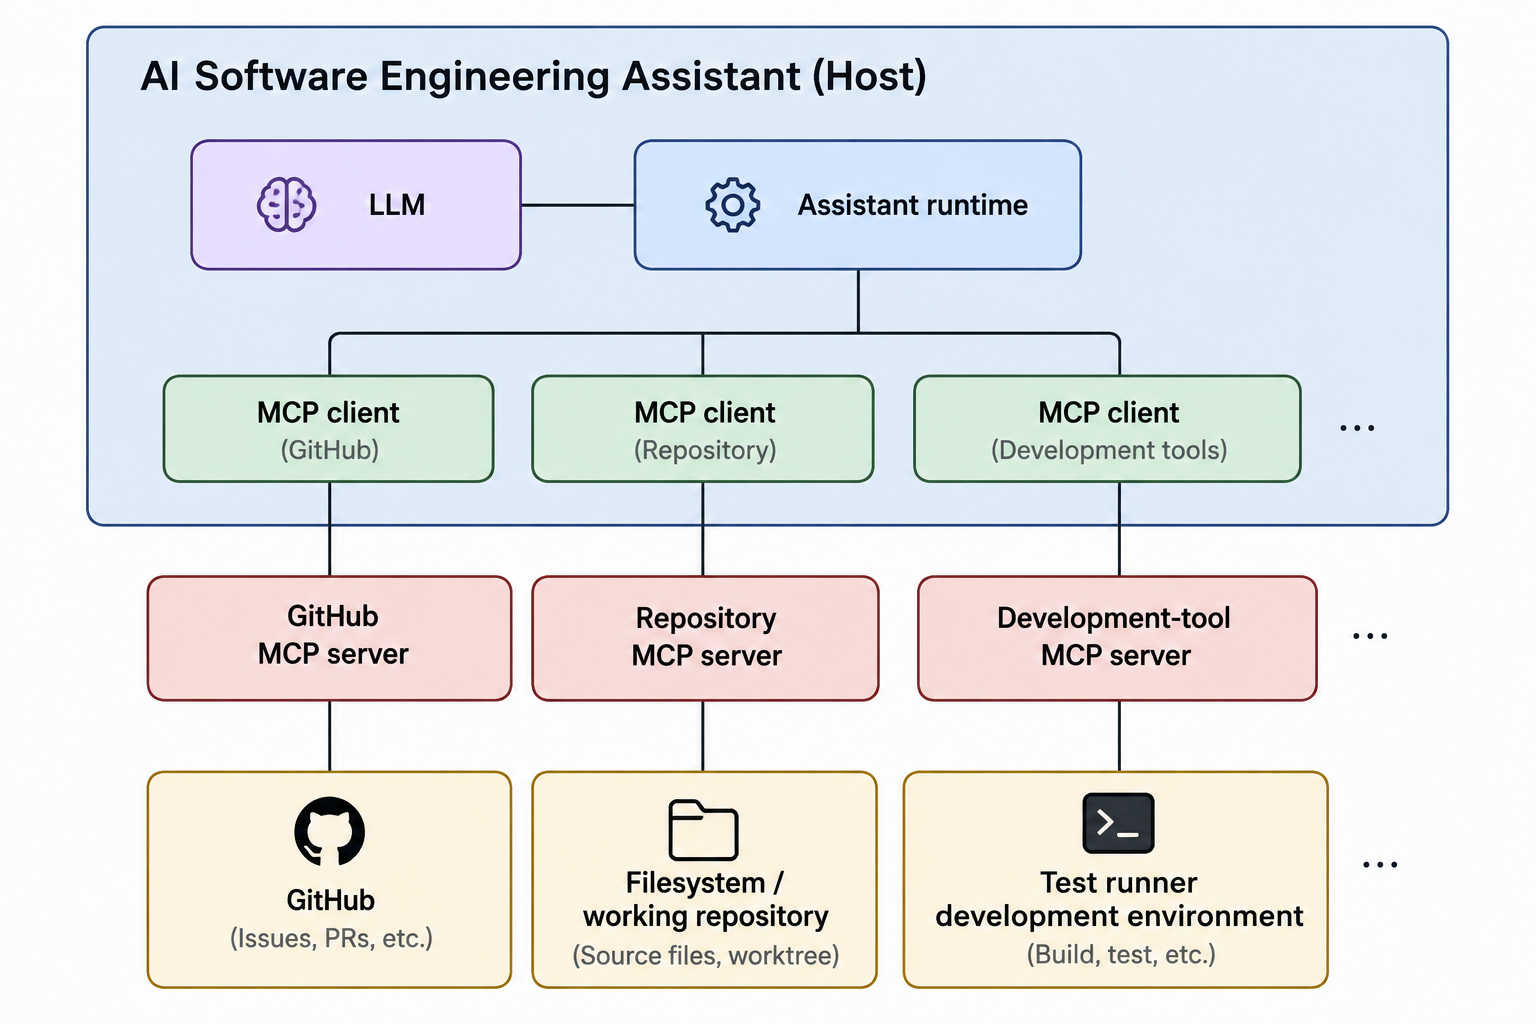
\includegraphics[width=\linewidth]{images/mcp-host-client-server.png}
\caption{Placement of MCP clients and servers between the AI Software Engineering Assistant and external systems.}
\label{fig:mcp-architecture}
\end{figure}

These server connections expose capabilities as \textbf{tools}, \textbf{resources} and \textbf{prompts}. Tools represent invocable operations, resources provide addressable data, and prompts provide reusable message templates. For the software-engineering workload considered here, tools and resources are most relevant because they provide access to executable operations and repository-related information.

MCP tool discovery should be distinguished from the tool-calling interface of the LLM. A server can describe a tool through its name, description and schema, but the model does not communicate with the MCP server directly. The Host selects which discovered tools are made available to the model and maps their definitions to the tool-calling interface of the selected inference runtime or model API. If the LLM generates a structured call such as \texttt{search\_code("Authorization")}, the assistant runtime maps it back to the corresponding MCP server. MCP therefore complements the function calling described in Chapter~\ref{chap:tool-use} rather than replacing it.

Figure~\ref{fig:mcp-tool-flow} follows a model-generated request through Host validation and MCP routing to backend execution, then returns the result for a subsequent model request.

\begin{figure}[!htbp]
\centering
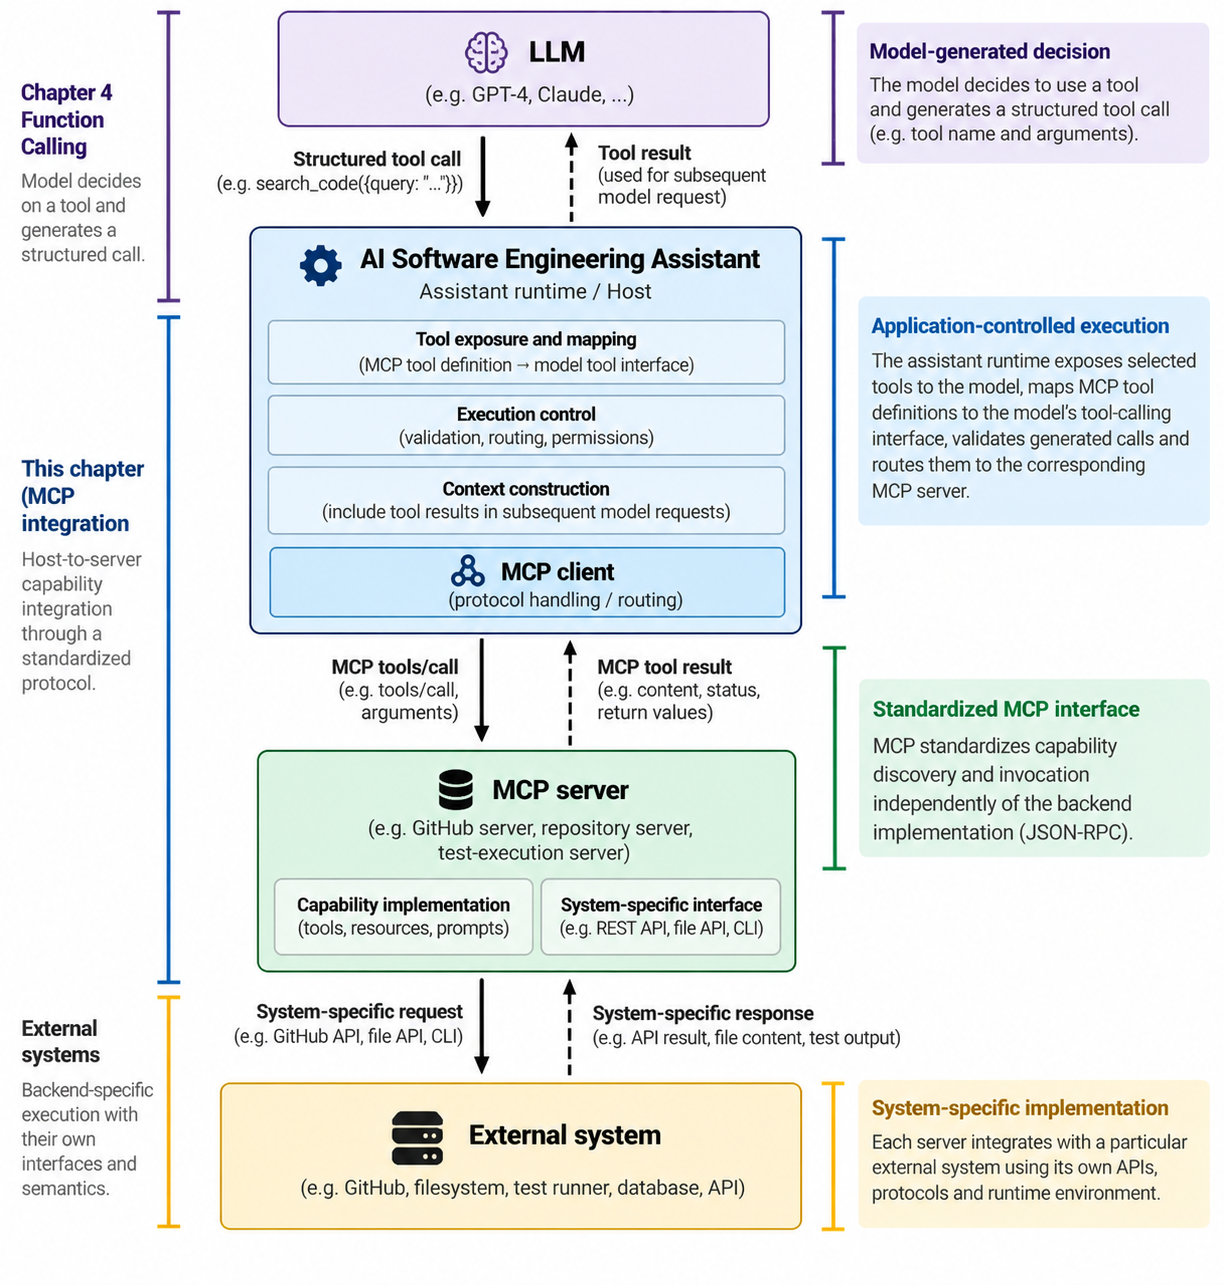
\includegraphics[width=\linewidth]{images/mcp-tool-execution-flow.png}
\caption{Flow from MCP tool discovery through model-visible tool selection to external tool execution and returned results.}
\label{fig:mcp-tool-flow}
\end{figure}

The set of capabilities exposed by a server, the subset selected by the Host and the tools actually included in a model request are separate concerns. When tool definitions are included in model requests, selecting a smaller task-relevant subset can reduce active-context usage and tool-selection ambiguity.

MCP uses JSON-RPC and supports both local and remote servers. This chapter refers to protocol revision \texttt{2026-07-28}, whose core uses self-contained requests rather than the protocol-level session lifecycle of earlier revisions \parencite{mcp2026architecture}. A stateless protocol core does not require the server or its operations to be stateless.

\section{MCP in the software engineering assistant}
\label{sec:mcp-assistant}

Consider again the task \emph{Fix GitHub issue \#42 and verify the solution}. The assistant needs the issue description, relevant repository information, the ability to modify the implementation and a way to verify the resulting code state. These capabilities may originate from independent systems while still being exposed through MCP.

A GitHub MCP server could provide operations for reading issue \#42 and creating a pull request. A repository or filesystem server could expose \texttt{read\_file}, \texttt{search\_code} and \texttt{apply\_patch}, while a test-execution MCP server could expose \texttt{run\_tests}. This allows heterogeneous backends to participate in one workflow without requiring the assistant runtime to implement each backend protocol directly.

A shared protocol does not create a shared workspace automatically. If repository inspection, modification and testing are handled by different servers, the Host must ensure that they refer to the intended repository, branch or working copy and to a consistent code state. A successful test result is relevant only if it verifies the version containing the changes being evaluated.

GitHub's official MCP server illustrates this approach by exposing GitHub functionality through configurable toolsets and individual tools. It can also operate in read-only mode, removing write operations exposed through that server \parencite{github-mcp-configuration}. Such configuration limits the GitHub integration but does not restrict capabilities provided by other independently configured servers.

MCP access should also be distinguished from retrieval and context construction. A server may expose a \texttt{search\_code} tool, but MCP does not define whether the underlying retrieval uses lexical search, embeddings or another strategy. Similarly, information returned through MCP does not automatically enter the LLM's active context. The assistant's context policy still determines which results are included, summarised or retained. MCP therefore standardises access, while retrieval determines what is found and context engineering determines what the model receives.

The same distinction applies to backend semantics. A GitHub MCP server may translate a tool call into GitHub API operations, while a filesystem server uses file APIs and a test-execution server starts a build or test process. MCP standardises capability exposure and invocation, not the behaviour of the underlying systems.

\section{Benefits, boundaries and production trade-offs}
\label{sec:mcp-tradeoffs}

The main architectural benefit of MCP is \textbf{reuse through a common integration boundary}. Backend-specific adapters still have to be implemented, but an MCP server can expose them to multiple compatible Hosts. Machine-readable discovery also allows a Host to obtain capability definitions without hard-coding every externally provided operation.

Protocol compatibility does not imply semantic uniformity. Two MCP servers may provide repository-search tools with different names, schemas, result structures or behaviour. Clear tool descriptions, bounded responsibilities and predictable results therefore remain important; MCP standardises the interaction mechanism but does not guarantee the quality of the interface.

The additional protocol boundary also introduces costs. Remote servers can add network latency, while separately deployed components introduce additional failure, versioning and observability concerns. These costs are useful when reuse or independent deployment matters, but a small system with a few fixed local operations may remain simpler with direct function integration.

MCP compatibility alone also does not establish a security boundary or make a connected server trustworthy. Isolation, authorisation and input validation must be enforced by the Host, server and deployment environment. Local servers are not automatically sandboxed, capabilities should follow least-privilege principles, and sensitive operations may require Host-controlled user approval \parencite{mcp2026security}.

MCP provides a reusable integration boundary through which heterogeneous external capabilities become available to the assistant. Coordinating those capabilities toward a task objective is the responsibility of the agents and agent harnesses examined in the following chapter.
